% !TeX encoding = UTF-8
% !TeX program = xelatex
% !TeX spellcheck = en_US

\documentclass{cjc}

\usepackage{booktabs}
\usepackage{siunitx}
\usepackage{hyperref}
\usepackage{nicematrix}
\usepackage{algorithm}
\usepackage{algorithmic}

\begin{document}

\title{基于x86多核处理器的高通量多元LDPC码FFT-SPA译码器的实现}
\author{Bertrand Le Gal\footnote{IMS Lab., Univ. Bordeaux, Bordeaux INP, CNRS UMR 5218, France} \and Christophe Jego\footnotemark[1]}

\maketitle

\begin{abstract}
  低密度奇偶校验(LDPC)码是一种众所周知的错误码,常被用于无线通信和卫星通信。
  而通过将LDPC码扩展到高阶伽罗瓦域,能够进一步提高其纠错性能,从而产生了所谓的
  多元LDPC码(NB-LDPC)。而纠错性能改进(CCSDS \citeyear{CCSDS_2014})是国际空间数据系统咨询委员
  会(CCSDS)在下一代上行链路实验规范(CCSDS \citeyear{CCSDS_2014}、\citeyear{CCSDS_2015})
  中采用NB-LDPC码的主要原因。NB-LDPC码对短帧具有较高的纠错效率,因此该码是物联网应用的理想选择。
  然而,这种性能上的增益是以解码计算复杂度为代价的(CCSDS \citeyear{CCSDS_2014}; CondeCanencia etal. \citeyear{comparison_NBLDPC})。
  本文给出了一个x86多核NB-LDPC译码器的实现。与GPU(图形处理单元)设备上最高效的
  工作相比,这一实现FFT-SPA算法的译码器的吞吐量提高了约1.3倍到2.7倍,延迟减少了
  95\%以上,功耗降低了一半。实际上,在x86架构上进行高效的内存映射和计算优化的话,
  可以实现比基于类似实验设置的GPU更高的解码吞吐量。因此,吞吐量效率、低功耗下的
  低处理延迟使得本文所提出的多核方案对于用于CCSDS标准和未来物联网应用中的SDR、
  Cloud-RAN系统中的NB-LDPC译码器的实时实现极具现实意义。\medskip\newline
  \textbf{关键字 }多元LDPC码,FFT-SPA,多核,SIMD,纠错码

\end{abstract}

\section{简介}

  纠错码(ECC)是现代数字通信系统中广泛用于提高系统可靠性的纠错技术。而低密度奇偶
  校验码\cite{gallager_low_1962}由于其接近信道容量的性能,成为了最流行的纠错码之一。
  许多卫星通信标准,如 DVB-S2X \cite{noauthor_dvb_nodate} 或 CCSDS \cite{CCSDS_2011},
  都采用了这种码族。文\cite{davey_low_1998,noauthor_barnault_nodate}提出了将二进制LDPC码扩展到多进制伽罗瓦域
  的方法,以提高纠错性能。这类方法很可能在未来的CCSDS标准中被采用\cite{CCSDS_2015,dolecek_non-binary_2014}。
  事实上,在CCSDS环境中,应用该方法后的纠错增益从1.0 dB提升到了1.3 dB\cite{CCSDS_2015}。
  因此,大量的研究集中在这一新的具有挑战性的代码系列上,例如高效的软件解码器实现\cite{noauthor_wang_nodate,noauthor_andrade_nodate,noauthor_beermann_nodate,andrade_optimized_2014,noauthor_thi_nodate,beermann_gpu_2015,noauthor_pham_nodate,liu_high-throughput_2018}
  或高效的硬件架构设计\cite{boutillon_design_2013,abassi_novel_2017}。
  然而,诸如灵活性、高吞吐量和低延迟等一系列面向未来基于SDR的系统的特性还有待进一步研究。

  ECC 技术通常用计算复杂度来区分。在过去的十年中,ASIC 或 FPGA是首选的实现方法,
  甚至对于地面基带站也是如此。实际上,基于 ASIC 的方案提供了最佳的面积、功耗和吞吐量特性。
  但是,它们的运行时灵活性低,开发周期长。为了解决这一问题,研究了基于FPGA的体系结构设计。
  而这些目标具有计算并行性强和低功耗的优点。然而,基于FPGA的硬件实现也具有有限的灵活性,
  并且设计周期也过长。另一方面,ASIC 和 FPGA 的实现都是基于近似的译码算法,
  这使得架构成本最小化的同时给纠错能力带来了负面影响。

  大规模并行可编程器件在获得很大进步和发展后,已被用于许多纠错码的译码器实现中,
  例如二进制LDPC码\cite{chang_accelerating_2011,falcao_portable_2012,noauthor_wang_nodate-1,li_efficient_2013,lin_high_2014,gal_high-throughput_2016,andrade_survey_2016}
  、NB-LDPC码\cite{noauthor_wang_nodate,noauthor_andrade_nodate,noauthor_beermann_nodate,andrade_optimized_2014,noauthor_thi_nodate,beermann_gpu_2015,noauthor_pham_nodate,liu_high-throughput_2018}
  和极性码\cite{noauthor_gal_nodate,gal_multi-gbs_2015,giard_low-latency_2018}。
  这些软件译码器的设计可达到Mbps或Gbps的吞吐量,也能够提供软件无线电(SDR)\cite{grayver_implementing_2013}
  系统所需的灵活性。

  许多最近的研究工作专注于NB-LDPC译码器在GPU设备上的软件实现\cite{noauthor_wang_nodate,noauthor_andrade_nodate,noauthor_beermann_nodate,andrade_optimized_2014,noauthor_thi_nodate,beermann_gpu_2015,noauthor_pham_nodate,liu_high-throughput_2018}。
  虽然二进制LDPC译码器在GPU和多核目标上的高效实现已经比较理想\cite{chang_accelerating_2011,falcao_portable_2012,noauthor_wang_nodate-1,li_efficient_2013,lin_high_2014,gal_high-throughput_2016,andrade_survey_2016},
  但是NBLDPC码却相去甚远。实际上,NB-LDPC译码算法与二进制LDPC译码算法有很大的不同。
  这意味着以前的优化策略不能直接移植。因此,针对GPU目标,研究人员提出了另外的并行化策略。
  由于解码算法的主要差异,还必须在多核体系结构上重新设计它们。第一批研究\cite{noauthor_andrade_nodate,noauthor_beermann_nodate,andrade_optimized_2014,beermann_gpu_2015,liu_high-throughput_2018}
  集中于在GPU目标上实现具有高纠错性能的NB-LDPC解码算法,用于只关注纠错性能的应用。
  使用5次分层译码迭代后,GPU上的吞吐率从1Mbps提高到了228Mbps。然而,处理延迟显著增加:
  当选择最有效的吞吐量设置时,延迟在21 ms到123 ms不等\cite{liu_high-throughput_2018}。
  第二批研究\cite{noauthor_wang_nodate,noauthor_thi_nodate,noauthor_pham_nodate}
  集中于在GPU设备上实现解码启发式算法。然而,即便有较低的计算复杂度,与基于初始公式的解码吞吐量相比,
  所实现的解码吞吐量仍不可观\cite{noauthor_andrade_nodate,liu_high-throughput_2018}。
  大多数基于GPU的解码器在吞吐量或延迟方面的低性能水平是由GPU的体系结构导致的,
  例如缓慢的全局内存、有限的共享内存等,及其相关的编程模型,这些限制造成映射NB-LDPC
  解码算法极具挑战性。

  本文详细介绍了另一种基于x86多核结构的NB-LDPC译码器的软件实现。本文选择FFT-SPA算法是因为它比最小和或SPA译码算法具有更低的计算复杂度和更高的纠错性能
  \footnote{尽管优化过的SPA和最小和译码器不是本文重点,但仍对其进行了实现和测试。在“实验”一章中有一栏对这些算法进行了性能比较。}。
  x86处理器的编程模型和结构特点与GPU不同。尽管与GPU设备相比,该算法的处理单元较少,
  但它似乎更好地利用了x86多核特性,就像其他ECC码族一样\cite{gal_high-throughput_2016,noauthor_wang_nodate-1,noauthor_cassagne_nodate}。
  此外,该解码器的吞吐量比大多数相关成果都要高\cite{noauthor_andrade_nodate,noauthor_beermann_nodate,andrade_optimized_2014,beermann_gpu_2015,liu_high-throughput_2018}。
  特别是在服务器级x86 CPU上,总能得到更好的吞吐量、延迟和功耗特性。
  为了达到这个性能水平,本文采用了不同的并行化策略和算法优化。实验结果表明,
  所提出的NB-LDPC软件译码器实现方案在吞吐量、延迟和能量消耗方面比基于GPU的实现更具竞争力。
  功耗的降低和低延迟的特性使得该实现更适合于SDR系统。与第一个借助OpenCL语言\cite{noauthor_wang_nodate}
  实现的x86软件解码器实现相比,本文提出的软件解码器实现直接利用了SIMD和多核特性,
  使其比\cite{noauthor_wang_nodate}中给出的x86实现快1000倍以上。

  论文的其余部分组织如下。第 \ref{sec:decoding} 节介绍了NB-LDPC码、FFT-SPA译码算法
  以及在GPU上实现NB-LDPC译码器的相关工作。然后,第 \ref{sec:fftspa} 节详细介绍了
  目标x86多核平台以及我们的并行化和优化方法。最后,在第 \ref{sec:experiment} 节中
  提供了性能分析和与相关工作的横向对比。

\section{NB-LDPC 码的译码}\label{sec:decoding}
\subsection{简介}

  $(N,K)$ NB-LDPC 码是一种由稀疏奇偶校验矩阵 $H$ 定义的线性分组码,其中非零元素属于
  $q\geq2$ \eqref{eq:1} 的伽罗瓦域$\mathbb{GF}(q)$。$H$矩阵的维数为$M{\times}N$,
  其中$M=N−K$是奇偶方程(或校验节点,CN)的数目,N是可变节点(VN)的数目,即码字中
  $\mathbb{GF}(q)$符号的数目。当$H$矩阵中的值$\alpha_{ij}$不为0时,
  $c_j$奇偶方程中就会带有元素$v_i$。第$j$行中非零元素的个数定义为用$d_{c_j}$表示的 CN 度。
  类似地,定义了第$i$列中非零元素的数量作为用$d_{v_i}$表示的 VN 度。

\begin{equation}\label{eq:1}
  \setlength{\arraycolsep}{3pt}
  H=
  \begin{pNiceMatrix}[first-row,first-col]
        & v_{0} & v_{1} & v_{2} & v_{3} & v_{4} & v_{5} & v_{6} & v_{7}\\
    c_0 & \alpha_{00} & \alpha_{10} & \alpha_{20} & 0 & 0 & 0 & 0 & 0 \\
    c_1 & 0 & 0 & 0 & \alpha_{31} & \alpha_{41} & \alpha_{51} & 0 & 0 \\
    c_2 & \alpha_{02} & 0 & 0 & \alpha_{32} & 0 & 0 & \alpha_{62} & 0 \\
    c_3 & 0 & \alpha_{13} & 0 & 0 & \alpha_{43} & 0 & 0 & \alpha_{73} \\
  \end{pNiceMatrix}
\end{equation}

  定义NB-LDPC码的$H$矩阵也可以用Tanner图表示,如图 \ref{fig:1} 所示。

\begin{figure}[htb]
  \centering
  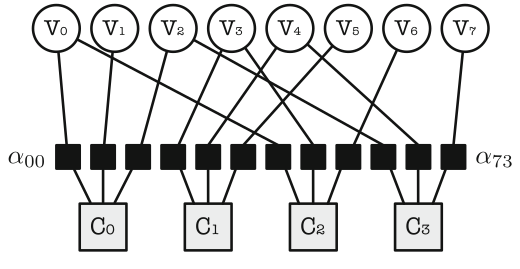
\includegraphics[width=\linewidth]{assets/fig1.png}
  \caption{Eq.\ref{eq:1}中 $H$ 矩阵的Tanner图}\label{fig:1}
\end{figure}

  码字由$x=\{x_0,x_1,\dots,x_{N-1}\}$表示,其中$x_i,i\in[0,N-1]$ 是由 $m=\log_2(q)$
  位表示的$\mathbb{GF}(q)$符号。为了描述等于$\mathbb{GF}$的$q$元素之一的符号$x$的概率$q$,
  使用 q 维 LR 向量。$x_i$的第 $a$ 个符号元素的概率由 $p_i(a),a\in[0,q-1]$ 表示。

  集合$\Psi(c_j)$表示奇偶校验方程$c_j$中包含的$x$个$d_{c_j}$符号。同样,集合$\Psi(x_i)$
  包含了含有符号$x_i$的$d_{v_i}$校验方程。排除由符号$/$表示,例如,$\Psi(x_i)/c_j$表示
  除$c_j$外的$\Psi(x_i)$检验方程组。

  与二进制 LDPC 译码类似,NB-LDPC 译码基于消息传递算法执行。最佳纠错性能是通过执行
  Sum-Product算法\cite{carrasco_non-binary_2008}(SPA)或其等效公式(如FFT-SPA\cite{carrasco_non-binary_2008})获得的。
  FFT-SPA 解码算法的优点之一,是由于去除消息卷积而使得处理 CN 的计算复杂度降低。
  这种改进是在不影响解码性能的情况下获得的,因为它们在数学上是等价的\cite{comparison_NBLDPC}。
  此外,如在\cite{noauthor_andrade_nodate}中强调并在\cite{carrasco_non-binary_2008}中演示的,
  大多数$\mathbb{GF}(q)$域的解码操作都被转移到了$\mathbb{R}$,以便于实现。

  算法1提供了用于水平分层解码调度的形式化FFT-SPA解码算法\cite{beermann_gpu_2015,liu_high-throughput_2018,noauthor_hocevar_nodate}。
  与基于泛洪的调度相比,它有助于:(i)在提供类似的纠错性能的同时加倍收敛速度;
  (ii)减少解码器的内存占用。这些特性使得这种计算调度在软件\cite{noauthor_thi_nodate,beermann_gpu_2015,noauthor_pham_nodate,liu_high-throughput_2018}
  和硬件\cite{boutillon_design_2013,abassi_novel_2017}实现中都很流行。

\begin{algorithm}[htb]
  \begin{algorithmic}[1]
    \STATE \textbf{Step 1}: 初始化
    \STATE $p_i(x)=p(v_i=x|y_i)$
    \STATE $m^0_{ji}(x)=1$
    \STATE $\vartriangleright$ 进行 $iter_max$ 次解码迭代
    \FORALL{$t=1\rightarrow(iter\_max)$}
      \STATE \textbf{Step 2}: 轮询 NB-LDPC 码中的所有 CN
      \FORALL{$j{\in}C$}
        \STATE$\vartriangleright$ 计算接收到的消息 $m_{ij}$
        \FORALL{$i\in\Psi(j)$}
          \STATE $m_{i j}^{t}(x)=\left(\sum_{x \in \mathbb{G} \mathbb{F}} m_{j i}^{t-1}(x)\right) \times\left(\frac{p_{i}(x)}{m_{j i}^{t-1}(x)}\right)$
          \STATE $M^t_{ij}=\Theta_{\alpha_{ij}}(m^t_{ij})$
          \STATE $\tilde{M^t_{ij}}=FFT(M^t_{ij})$
        \ENDFOR
        \STATE$\vartriangleright$傅里叶域中累乘概率
        \FORALL{$i\in\Psi(j)$}
          \STATE $\tilde{M}_{j i}^{t}=\prod_{i^{\prime} \in \Psi(j) / i} \tilde{M}_{i^{\prime} j}^{t}$
        \ENDFOR
        \STATE$\vartriangleright$计算输出的消息 $m_{ij}$
        \FORALL{$i\in\Psi(j)$}
          \STATE $M^t_{ji}=FFT^{-1}(\tilde{M^t_{ji}})$
          \STATE $m^t_{ji}=\Theta^{-1}_{\alpha{ij}}(M^t_{ji})$
        \ENDFOR
        \STATE$\vartriangleright$更新符号概率
        \FORALL{$i\in\Psi(j)$}
          \STATE $p_i(x)=p_i(x)\times(\frac{m^t_{ji}(x)}{m^{t-1}_{ji}(x)})$
        \ENDFOR
      \ENDFOR
    \ENDFOR
    \STATE\textbf{Step 3}: 符号硬判
    \FORALL{$i\in{V}$}
      \STATE $\hat{v}_{i}=\arg \max \left(p_{i}(x)\right)$
    \ENDFOR
  \end{algorithmic}
  \caption{ 水平 TDMP FFT-SPA 算法}
  \label{alg:1}
\end{algorithm}

  该算法可以概括为三个主要步骤。首先,使用 $y_i$ 信道信息计算 $N$ 个接收符号 $p_i$ 的概率
  (算法1:行2)。对于每个符号 $p_i$,估计每个元素$x\in\mathbb{GF}(q)$的概率。
  其次,对 $H$ 矩阵中的所有 CN 依次求值(算法1:行7:27)。对于 CN 计算,首先动态
  计算从 VN 到 CN 的 $m_{ij}$ 消息。然后,生成 $m_{ji}$ 消息并更新每个符号
  $p_i(x)$ 的概率。最后,对于每个 $p_i(x)$,选择具有最高概率$p_i(x)$ 的符号
  $\tilde{v}_v$(算法1:行30:32)。

  重复包括顺序处理 CN 的第二步,直到达到最大迭代次数或获得有效码字为止。CN 处理可扩展为7个基本阶段:
\begin{enumerate}
  \item 从 VN 到 CN 的消息 $m^t_{ij}(x)$ 是根据当前 VN 值($p_i(x)$)和从上一次
  迭代中从 CN 到 VN 的消息($m^{t-1}_{ji}(x)$)进行动态计算。
  \item 消息 $m_{ij}$ 在 $\mathbb{GF}$ 域中与来自 $H$ 矩阵的 $\alpha_{ij}$ 值相乘。
  此操作等效于受 $\alpha_{ij}$ 约束的数据置换,表示为 $\Theta_{\alpha_{ij}}$。
  \item 然后使用 $FFT$ 变换操作,$M_{ij}$ 消息值被转换到傅里叶域。
  \item 在$\tilde{M}_{ij}$消息值之间的进行一组标量乘法产生 CN 到 VN 消息。
  \item 通过 $FFT^{-1}$ 变换操作,消息值被转回概率域。 
  \item 消息 $M_{ji}$ 在 $\mathbb{GF}$ 域中除以第 2 阶段中使用的 $\alpha_{ij}$ 值。
  \item 最后,根据计算出的 $m^t_{ji}(x)$ 值来更新符号概率 $p_i(x)$。
\end{enumerate}

  在解码过程中,解码器只需要存储 $N$ 个 $p_i$ 元素和 $M\times{d_{c_j}}$ 个 $m_{ji}$ 元素。
  实际上,在第 $t−1$ 次迭代中用于存储的元素 $m^{t-1}_{ji}$ 的内存可以被重用于
  在第 $t$ 次迭代中存储元素 $m^t_{ji}$。注意,元素 $p_i$ 和 $m_{ji}$ 本质上由 $q$ 元素构成。

\subsection{相关工作}
  
  为了提供实现灵活性和高吞吐量性能,最近的许多研究都集中在将 NB-LDPC 解码器映射到 GPU 设备上\cite{noauthor_wang_nodate,noauthor_andrade_nodate,noauthor_beermann_nodate,andrade_optimized_2014,noauthor_thi_nodate,beermann_gpu_2015,noauthor_pham_nodate,liu_high-throughput_2018}。
  这些研究的目的是利用 GPU 设备提供的大量计算并行度来达到高吞吐量,就像之前对二进制
  LDPC 解码所做的那样\cite{li_efficient_2013,lin_high_2014,gal_high-throughput_2016}。
  实际上,为了使软件方案适用于数字通信系统仿真或 SDR 目的,必须解决灵活性、吞吐量、延迟和功耗效率等问题。

  第一批工作\cite{noauthor_andrade_nodate,noauthor_beermann_nodate,andrade_optimized_2014,beermann_gpu_2015,liu_high-throughput_2018}
  专注于基于 SPA 的算法,以提供高纠错性能。为了降低解码过程的计算复杂度,FFT-SPA \cite{noauthor_andrade_nodate}
  解码算法是首选。实际上,在 CN 处理中引入的 FFT 运算将 SPA 算法的卷积运算转化为一组标量项的乘积。
  CN 处理的计算复杂度原来是$O(M\times3\times(d_c−2)\times2^{2{\times}m})$,现在降低
  到$O(M\times{d_c}\times{m}\times2^{m})$\cite{declercq_decoding_2007}。
  文献\cite{noauthor_andrade_nodate}中报告的第一个基于 GPU 的实现在执行 10 次泛洪迭代时,
  $\mathbb{GF}(256)$ NB-LDPC 码的吞吐量在 0.5 到 1.6 Mbps 之间。由于 FFT 处理中计算并行性的降低,
  所以 $q$ 值较低时吞吐量也较低。这实际上限制了 GPU 核心的使用率,从而进一步
  限制了解码器的全局效率。\cite{noauthor_beermann_nodate}中也报告了类似的结论。
  注意,这项工作的第一个目标是支持不规则的 NB-LDPC 码。在\cite{beermann_gpu_2015}中,
  详细介绍了基于 FFT-SPA 算法分层公式的 NB-LDPC 解码器的实现。与\cite{noauthor_beermann_nodate}
  中提到的方法相比,它增加了解码吞吐量,从而实现了等效的纠错性能。
  然而,对于 $\mathbb{GF}(16)$ 到 $\mathbb{GF}(256)$ NB-LDPC 码,所测量的解码
  吞吐量仍然低于 0.5 Mbps。最近,在\cite{liu_high-throughput_2018}中提出了一种高效的
  基于 GPU 的解码器实现。在考虑 GPU 特性的基础上,找到了 FFT-SPA 译码算法的有效映射。
  基于分层的调度与高端 GPU 设备的组合使得能够针对 $\mathbb{GF}(16)$ NB-LDPC 码获得
  228 Mbps 的峰值吞吐量和 123 ms 的处理延迟。

  第二批工作\cite{noauthor_wang_nodate,noauthor_thi_nodate,noauthor_pham_nodate}
  集中于 SPA 解码算法的简化版本。不过,SPA 和 FFT-SPA 解码算法由于其高计算复杂度
  而不满足硬件结构设计约束。此后,为了便于 NB-LDPC 译码器的硬件实现,提出了一些
  低复杂度的译码算法:MinSum\cite{declercq_decoding_2007}、Min-Max\cite{declercq_decoding_2007}
  和 Extended Min-Sum\cite{noauthor_voicila_nodate}。在这些译码算法中,$\mathbb{R}$中
  的乘法和除法运算被转换成加法、减法和最小/最大运算。一些基于 GPU 的实现\cite{noauthor_wang_nodate,noauthor_thi_nodate,noauthor_pham_nodate}
  侧重于 min-max 解码技术。事实上,低计算复杂度似乎更好地映射到GPU设备上。需要注意的是,
  与基于 SPA 的算法相比,min-max 算法对纠错性能也有负面影响。然而,即使具有较低的计算复杂度,
  对于 $\mathbb{GF}(32)$ NB-LDPC 码,GPU 实现也未能达到高于 0.7 Mbps 的吞吐量。
  这种效率问题来自于 CN 计算中涉及的卷积式处理。

  总的来说,在 GPU 实现的相关工作表明,NB-LDPC 译码过程具有较高的计算并行度。
  因此,,它可以借助多核实现加速。然而,与 GPU 设备相关联的架构约束和编程模型似乎
  限制了 NB-LDPC 解码器在解码吞吐量和延迟方面的实现效率。因此,在本文中,我们重点
  讨论了这样一个多核体系结构,它提供了不同的编程模型和其他体系结构约束。实验结果表明,
  NB-LDPC 译码算法的计算并行度非常适合 x86 处理器。

\section{FFT-SPA 算法实现}\label{sec:fftspa}
\subsection{选定的多核架构}

  多核设备(例如 x86 或 ARM 处理器)提供足够当前的处理资源,以达到 Mbps 或 Gbps 吞吐量性能。
  如二进制 LDPC 码\cite{gal_high-throughput_2016,gal_high-throughput_2015}解码所示,
  它们应该适用于大多数 SDR 系统。所有的现代处理器都提供单指令多数据(SIMD)功能,
  使得在不同的数据集上同时执行 $Q$ 个相同的计算。例如,在当前的 x86 处理器中,
  使用 AVX2 配置,可以用一条指令处理 $Q=8$ 浮点计算。注意,根据功能单元的使用情况,
  时钟周期可以触发多条指令。目前,x86 处理器内核最多可以并发执行 6 条指令。这种
  并行化方法主要适用于不需要条件语句或分支语句的情况下,大量数据需要相同处理的计算序列。
  此外,还可以使用多指令多数据(MIMD)功能。它为不同的计算序列或程序在不同的数据集
  上并行执行提供了机会。因此,它使得并行帧处理成为可能。下一节将详细介绍
  利用 SIMD 和 MIMD 特性提出的 FFT-SPA 实现和优化选择\footnote{实现NB-LDPC 译码器的源代码将会在 GitHub 上开源}。

\subsection{并行化策略}

三种主要的SIMD并行化策略可以加速基于MP的算法:
\begin{itemize}
  \item $S_1$ 策略包括并行解码多个帧,如\cite{gal_high-throughput_2016,gronroos_efficient_2012}
  中的二进制LDPC解码器。它提供了处理和内存访问规则,从而提高了吞吐量性能。尽管如此,
  它依然引入了处理延迟(至少是$Q$倍)和巨大的内存占用。
  \item $S_2$ 策略包括跨 CN 内核的并行计算,例如并行处理 $Q$ 个 CN 内核。该策略缺乏内存访问规则性,
  需要对 CN 内核进行特殊的调度。其实,并行执行的 CN 可以访问不同的 VN 元素。
  \item $S_3$ 策略包括对单个CN内核的并行计算。对于二进制LDPC解码器的软件实现,
  由于CN元素的计算复杂度较低,$S_3$策略被丢弃\cite{gal_high-throughput_2016}。
  不过,对于NB-LDPC译码算法,由于$\mathbb{GF}(q),q\geq{Q}$,CN核的计算复杂度很高,
  并且内存访问是规则的。因此,它使$S_3$策略更为合适。
\end{itemize}

  为了获得最佳的灵活性、吞吐量和延迟平衡,本文放弃了$S_1$和$S_2$并行化策略。
  由于对于所有的NB-LDPC码,不可能实现避免VN访问冲突的CN重排步骤。所以只研究了$S_3$策略。

\begin{table}[htb]
  \caption{\\根据$d_c$归一化后的 CN 处理时间复杂度估计及并行可能性}
  \label{tab:1}
  \setlength\tabcolsep{3pt}% 调整列间距
  \begin{tabular}{cccccc}
    \toprule
    算法1 & 处理任务 & 加/减 & 乘 & 除 & ECN \\
    \midrule
    L.10  & 消息处理 & - & - & \blue{$q$} & - \\
    L.10  & 消息归一化 & \red{$q-1$} & - & \blue{$q$} & - \\
    L.11  & $\mathbb{GF}$中的累乘 & - & - & - & - \\
    L.12  & $FFT$ 处理 & \red{$q.\log_2(q)$} & - & - & - \\
    L.20  & $FFT^{-1}$ 处理 & \red{$q.\log_2(q)$} & - & - & - \\
    L.21  & $\mathbb{GF}$中的除法 & - & - & - & - \\
    L.25  & 更新 VN 值 & - & \blue{$q$} & \blue{$q$} & - \\
    L.16  & 频域中的 CN & - & - & - & \red{$3.(d_c-2)$} \\
    -     & ECN & - & \blue{$q$} & - & - \\
    \bottomrule
  \end{tabular}
\end{table}

\begin{table}[htb]
  \caption{\\根据$d_c$归一化后的 CN 处理空间复杂度估计及并行可能性}
  \label{tab:2}
  \setlength\tabcolsep{4.5pt}% 调整列间距
  \begin{tabular}{ccccc}
    \toprule
    算法1 & 处理任务 & 加载 & 保存 & 存储的数据 \\
    \midrule
    L.10  & 消息处理 & \blue{$2.q$} & \blue{$q$} & $q$ \\
    L.10  & 消息归一化 & \blue{$q$} & \blue{$q$} & $2.q$ \\
    L.11  & $\mathbb{GF}$中的累乘 & \red{$q$} & \blue{$q$} & $q$ \\
    L.12  & $FFT$ 处理 & \blue{$q$} & \blue{$q$} & $q.\log_2(q)$ \\
    L.20  & $FFT^{-1}$ 处理 & \blue{$q$} & \blue{$q$} & $q.\log_2(q)$ \\
    L.21  & $\mathbb{GF}$中的除法 & \red{$q$} & \blue{$q$} & $q$ \\
    L.25  & 更新 VN 值 & \blue{$3\times{q}$} & \blue{$q$} & $q$ \\
    L.16  & 频域中的 CN & - & - & $3q.(d_c-2)$ \\
    -     & ECN & \blue{$2.q$} & \blue{$q$} & $q$ \\
    \bottomrule
  \end{tabular}
\end{table}

\section{实验结果}\label{sec:experiment}
\subsection{二级标题}

\subsubsection{三级标题}

正文部分, 字体为5号宋体。

文件排版采用 TeX Live。

正文文字要求语句通顺,无语法错误,结构合理,条理清楚,不影响审稿人、读者阅读理解全文内容。以下几类问题请作者们特别注意:

1)文章题目应明确反映文章的思想和方法;文字流畅,表述清楚;

2)中文文字、英文表达无语法错误;

3)公式中无符号、表达式的疏漏,没有同一个符号表示两种意思的情况;

4)数学中使用的符号、函数名用斜体;

5)使用的量符合法定计量单位标准;

6)矢量为黑体,标量为白体;

7)变量或表示变化的量用斜体;

8)图表规范,量、线、序无误,位置正确(图表必须在正文中有所表述后出现,即…如图1所示)(注意纵、横坐标应有坐标名称和刻度值)。

9)列出的参考文献必须在文中按顺序引用,即参考文献顺序与引用顺序一致,各项信息齐全(格式见参考文献部分);

10)首次出现的缩写需写明全称,首次出现的符号需作出解释。

11)图的图例说明、坐标说明全部用中文或量符号。

12)图应为矢量图。

13)表中表头文字采用中文。

14)公式尺寸:

标准:10.5磅

下标/上标:5.8磅

次下标/上标:4.5磅

符号:16磅

次符号:10.5磅

15)组合单位采用标准格式,如:“pJ/bit/m4”应为“\si{pJ/(bit.m^4)}”


\begin{theorem}
  定理内容。
  “定义”、“假设”、“公理”、“引理”等的排版格式与此相同,详细定理证明、公式可放在附录中。
\end{theorem}

\begin{proof}
  证明过程.* [“例 x”等的排版格式相同]
\end{proof}

\begin{figure}[htb]
  \centering
  \includegraphics[width=\linewidth]{example-fig.pdf}
  \caption{图片说明 *字体为小 5 号,图片应为黑白图,图中的子图要有子图说明*}
\end{figure}

\begin{table}[htb]
  \centering
  \caption{表说明 *表说明采用黑体*}
  \small
  \begin{tabular}{cc}
    \toprule
    示例表格 & 第一行为表头,表头要有内容 \\
    \midrule
             &                            \\
    \midrule
             &                            \\
    \bottomrule
  \end{tabular}
\end{table}

% \begin{procedure}
%   定理内容。
%   “定义”、“假设”、“公理”、“引理”等的排版格式与此相同,详细定理证明、公式可放在附录中。
% \end{procedure}

% \begin{algorithm}
%   定理内容。
%   “定义”、“假设”、“公理”、“引理”等的排版格式与此相同,详细定理证明、公式可放在附录中。
% \end{algorithm}



\section*{致谢}

致谢内容。


\nocite{*}

\bibliographystyle{cjc}
\bibliography{refs}



\appendix

\section{}

附录内容置于此处,字体为小5号宋体。附录内容包括:详细的定理证明、公式推导、原始数据等



% \begin{background}
% *论文背景介绍为英文,字体为小5号Times New Roman体*

% 论文后面为400单词左右的英文背景介绍。介绍的内容包括:

% 本文研究的问题属于哪一个领域的什么问题。该类问题目前国际上解决到什么程度。

% 本文将问题解决到什么程度。

% 课题所属的项目。

% 项目的意义。

% 本研究群体以往在这个方向上的研究成果。

% 本文的成果是解决大课题中的哪一部分,如果涉及863/973以及其项目、基金、研究计划,注意这些项目的英文名称应书写正确。
% \end{background}

\end{document}
